\documentclass{article}

\usepackage{graphicx,wrapfig,color}

\newcommand{\progname}{\textsc{PyFEM}}

\title{\textsc{PyFEM} X.Y\\
\vspace{1cm}
User manual}
\author{Joris J.C. Remmers, Clemens V. Verhoosel and Ren\'e de Borst}

\renewcommand{\arraystretch}{1.5}

\usepackage{fancybox}
\newcounter{grayboxCounter}[section]

\definecolor{gray}{rgb}{0.7,0.7,0.7}
\definecolor{mygray}{gray}{0.9}

\newenvironment{graybox}{

\begin{center}\noindent\ignorespaces\begin{Sbox}\begin{minipage}{10cm}}%
{\end{minipage}\end{Sbox}%
\fcolorbox{black}{mygray}{\TheSbox}\vspace{5mm}\ignorespacesafterend\end{center}}

\begin{document}

\maketitle

\tableofcontents

\section{About the code}

This is the user manual for \progname~version X.Y. This \texttt{python}-based finite element code 
accompanies the book:                                              
          
\vspace{3mm}                                                       
\noindent         
'Non-Linear Finite Element Analysis of Solids and Structures' by      
 R. de Borst, M.A. Crisfield, J.J.C. Remmers and C.V. Verhoosel.        
 John Wiley and Sons, 2012, ISBN 978-0470666449                        

\begin{figure}[h]
\centering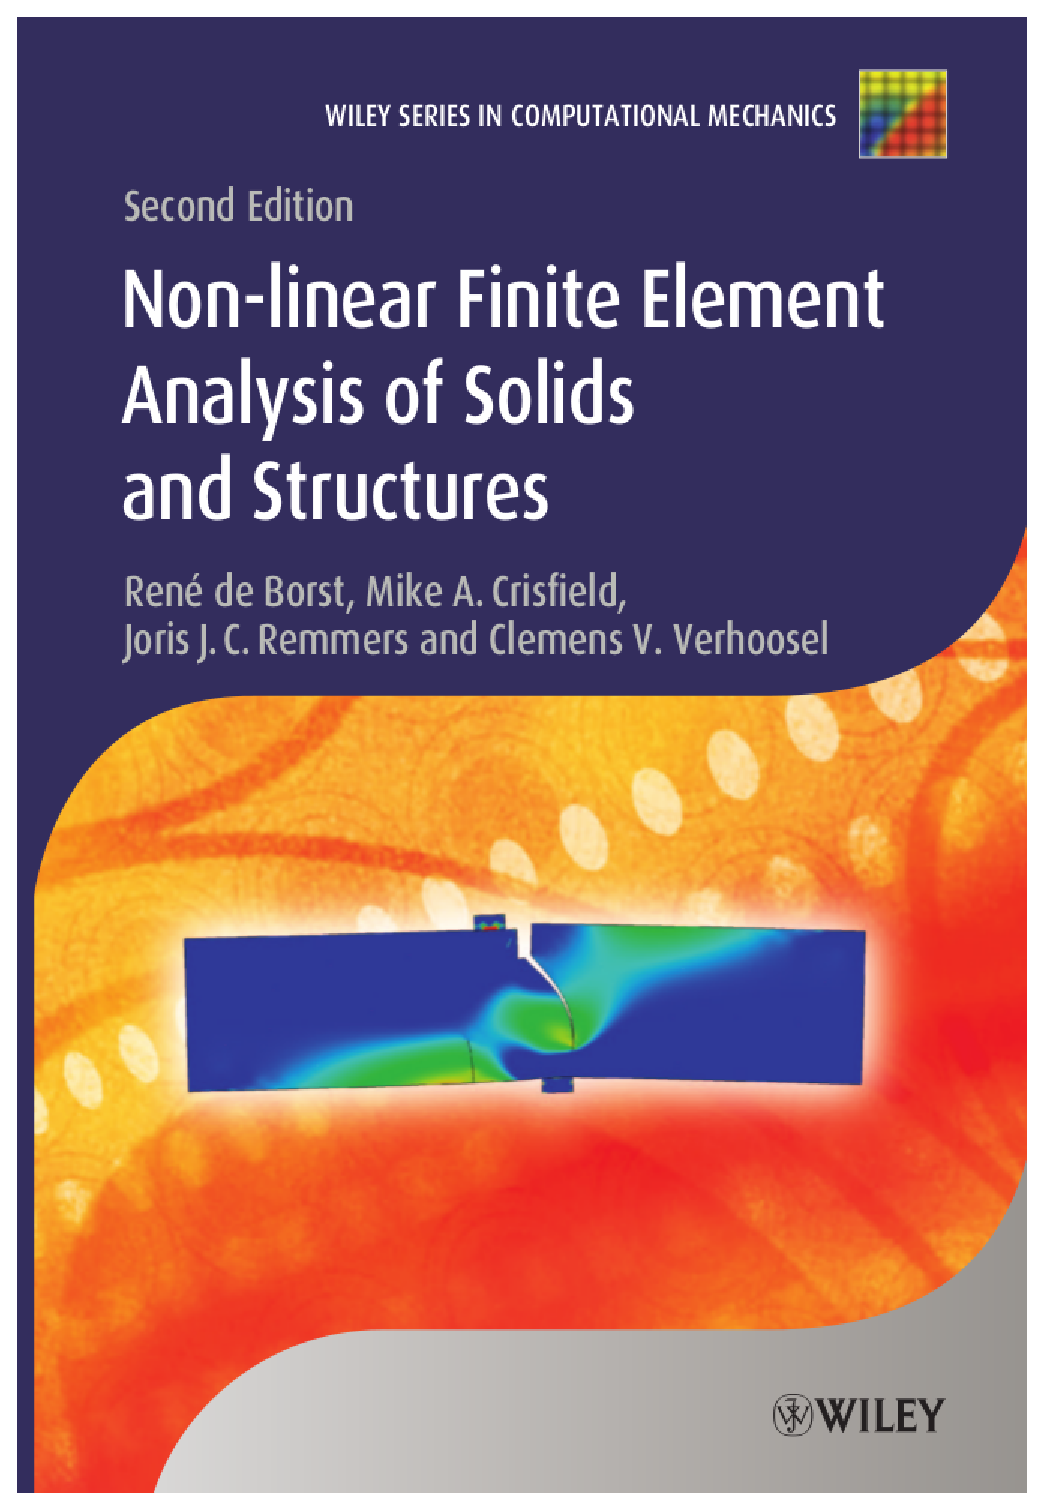
\includegraphics[width=0.5\textwidth]{img/cover.eps}
\end{figure}
                                                                          
\noindent
The code is open source and intended for educational and scientific     
purposes only. If you use \progname~in your research, the developers would 
be grateful if you could cite the book in your work. Comments and suggestions
are welcome at:
\begin{verbatim}
  PyFEM-support@tue.nl                                                                                                
\end{verbatim}
                                                                          
\subsection*{Disclaimer}

\noindent
The authors reserve all rights but do not guarantee that the code is    
free from errors. Furthermore, the authors shall not be liable in any   
event caused by the use of the program.                                 

\section{Installation}

The code can be downloaded from the website that accompanies the book.

\begin{verbatim}
  http://www.wiley.com/go/deborst
\end{verbatim}
\noindent
On this website, both the current version X.Y as well as all previous major releases of the code
can be found. The code is packed as a \texttt{.zip} or a \texttt{.tar.gz} file and 
can be unzipped in a directory of choice. 

This version of the \progname~is written to work properly in combination with 
\texttt{python} version 3.x. In addition, the code uses the modules \texttt{numpy}, \texttt{scipy} and
\texttt{matplotlib}. Installation guidelines are given for various operating systems.

\subsection{Windows OS (Windows XP and Windows 7)}

\begin{enumerate}
\item Since precompiled versions of \texttt{numpy}, \texttt{scipy} and 
\texttt{matplotlib} are available in 32-bit versions only, it
is advised to install the 32-bit version of \texttt{python}. This code is available
at:
\begin{verbatim}
  http://www.python.org/getit
\end{verbatim} 
It is recommended to install the latest version 3.x.
\item Download and install \texttt{numpy}.
This module is available at:
\begin{verbatim}
  http://sourceforge.net/projects/numpy/files/NumPy
\end{verbatim}
It is recommended to install the latest 32-bit version, which is 1.6.2.
\item Download and install \texttt{scipy}.
This module is available at:
\begin{verbatim}
  http://sourceforge.net/projects/scipy/files/scipy/
\end{verbatim}
It is recommended to install the latest 32-bit version, which is 0.11.01b.
\item Download and install \texttt{matplotlib}.
This module is available at:
\begin{verbatim}
  http://sourceforge.net/projects/matplotlib/files/matplotlib/
\end{verbatim}
It is recommended to install the latest 32-bit version, which is version 1.1.0.
\item Run the python file \texttt{install.py} in the root directory 
\texttt{pyfem-X.Y} by double-clicking it. It creates the required executables 
and returns the total path in which \progname~is installed. This path must be 
added to the environment variables \texttt{PYTHONPATH} and \texttt{PATH}. 

Windows has a built-in dialog for changing environment variables. In the case of Windows XP in
the classical view:
\begin{itemize} 
\item Click your machine (usually located on your Desktop 
and called “My Computer”) and choose Properties there. 
\item Then, open the Advanced tab and click the Environment 
Variables button.
\end{itemize} In short, your path is:
\begin{verbatim}
  My Computer->Properties->Advanced->Environment Variables
\end{verbatim}
In this dialog, you can add or modify user and system variables. 
To change system variables, you need non-restricted access to your machine (i.e. Administrator rights).

The main program \texttt{pyfem} can be run from the command prompt. For example, in order to run the
file \texttt{StressWave20x20.pro} in the directory \texttt{examples\textbackslash ch05}, simply type:
\begin{verbatim}
  pyfem StressWave20x20.pro
\end{verbatim}
or by clicking any \texttt{.pro} file with the right mouse button and selecting the batch file \texttt{pyfem.bat} 
to execute it with.
\end{enumerate}

\subsection{Linux OS}

The \texttt{python} program and the modules \texttt{numpy}, \texttt{scipy} and \texttt{matplotlib}
are included in most common distributions of Linux and can be installed without any problems. In many
cases, different versions of \texttt{python} are offered. Please make sure that \texttt{python} version 3.6 or higher is
installed.

\noindent Run de \texttt{python} file \texttt{install.py} in the root directory 
\texttt{pyfem-X.Y}. In a terminal, one can type:
\begin{verbatim}
  python install.py
\end{verbatim}
This script returns the total path in which \progname~is installed. This path must be 
added to the environment variables \texttt{PYTHONPATH} and \texttt{PATH}. When using a bash shell, 
the following lines have to be added to the file \texttt{.bashrc} in your root directory:
\begin{verbatim}
  export PYTHONPATH=<pyfemdir>
  alias  pyfem="python <pyfemdir>/PyFEM.py"
\end{verbatim}
When using csh or tcsh add the following lines to \texttt{.cshrc} or \texttt{.tcshrc}:
\begin{verbatim}
  setenv PYTHONPATH <pyfemdir>
  alias  pyfem "python <pyfemdir>/PyFEM.py"
\end{verbatim}
It goes without saying that in the case of multiple \texttt{PYTHONPATH} settings, the path to \progname~ 
should be added to existing paths. For example, in the case of a bash shell, this will look like:
\begin{verbatim}
  export PYTHONPATH=<pyfemdir>:$PYTHONPATH
\end{verbatim}
The main program \texttt{pyfem} can be run from the command prompt. For example, in order to run the
file \texttt{StressWave20x20.pro} in the directory \texttt{examples/ch05}, simply type:
\begin{verbatim}
  pyfem StressWave20x20.pro
\end{verbatim}

\subsection{Mac OS}

\begin{enumerate}
\item The most recent versions of Apple Mac-OS ship with their own version of \texttt{python}. However, it is 
strongly recommended to install the official \texttt{python} 3.x at: 
\begin{verbatim}
  http://www.python.org/getit
\end{verbatim} 
The latest version is 3.x
\item Download and install the latest version of \texttt{numpy}.
This module is available at:
\begin{verbatim}
  http://sourceforge.net/projects/numpy/files/NumPy
\end{verbatim}
It is recommended to install the latest version, which is 1.6.2.
\item Download and install \texttt{scipy}.
This module is available at:
\begin{verbatim}
  http://sourceforge.net/projects/scipy/files/scipy/
\end{verbatim}
It is recommended to install the latest version, which is 0.11.01b.
\item Download and install \texttt{matplotlib}.
This module is available at:
\begin{verbatim}
  http://sourceforge.net/projects/matplotlib/files/matplotlib/
\end{verbatim}
It is recommended to install the latest version, which is version 1.1.0.
\item When all programs and packages mentioned above are installed, open a terminal and run 
the \texttt{python} file \texttt{install.py} in the root directory \texttt{pyfem-X.Y}, by typing:
\begin{verbatim}
  python install.py
\end{verbatim}
This script returns the total path in which \progname~is installed. This path must be 
added to the environment variables \texttt{PYTHONPATH} and \texttt{PATH}. The following lines 
have to be added to the file \texttt{.bashrc} in your root directory:
\begin{verbatim}
  export PYTHONPATH="your_pyfem_path"
  alias  pyfem     ="python your_pyfem_path/PyFEM.py"
\end{verbatim}
\end{enumerate}

\subsection{Additional software}

\progname~can store the solution of a simulation in the \texttt{vtk}-format, which can be viewed with the 
program \textsc{Paraview}. This program is available for free for academic use from the following 
website\footnote{Please read the terms on their website in case of non-academic use.}:
\begin{verbatim}
  http://www.paraview.org
\end{verbatim} 
The results are stored as a single \texttt{.pvd} file, which refers to a number of \texttt{.vtu} files. By opening
the \texttt{.pvd} file in \textsc{Paraview} one can see the deformed mesh and stress contours, as shown in 
Figure~\ref{fig:stress}. A more detailed description how to create these output files is given in paragraph~\ref{par:vtk}.

\begin{figure}
\centering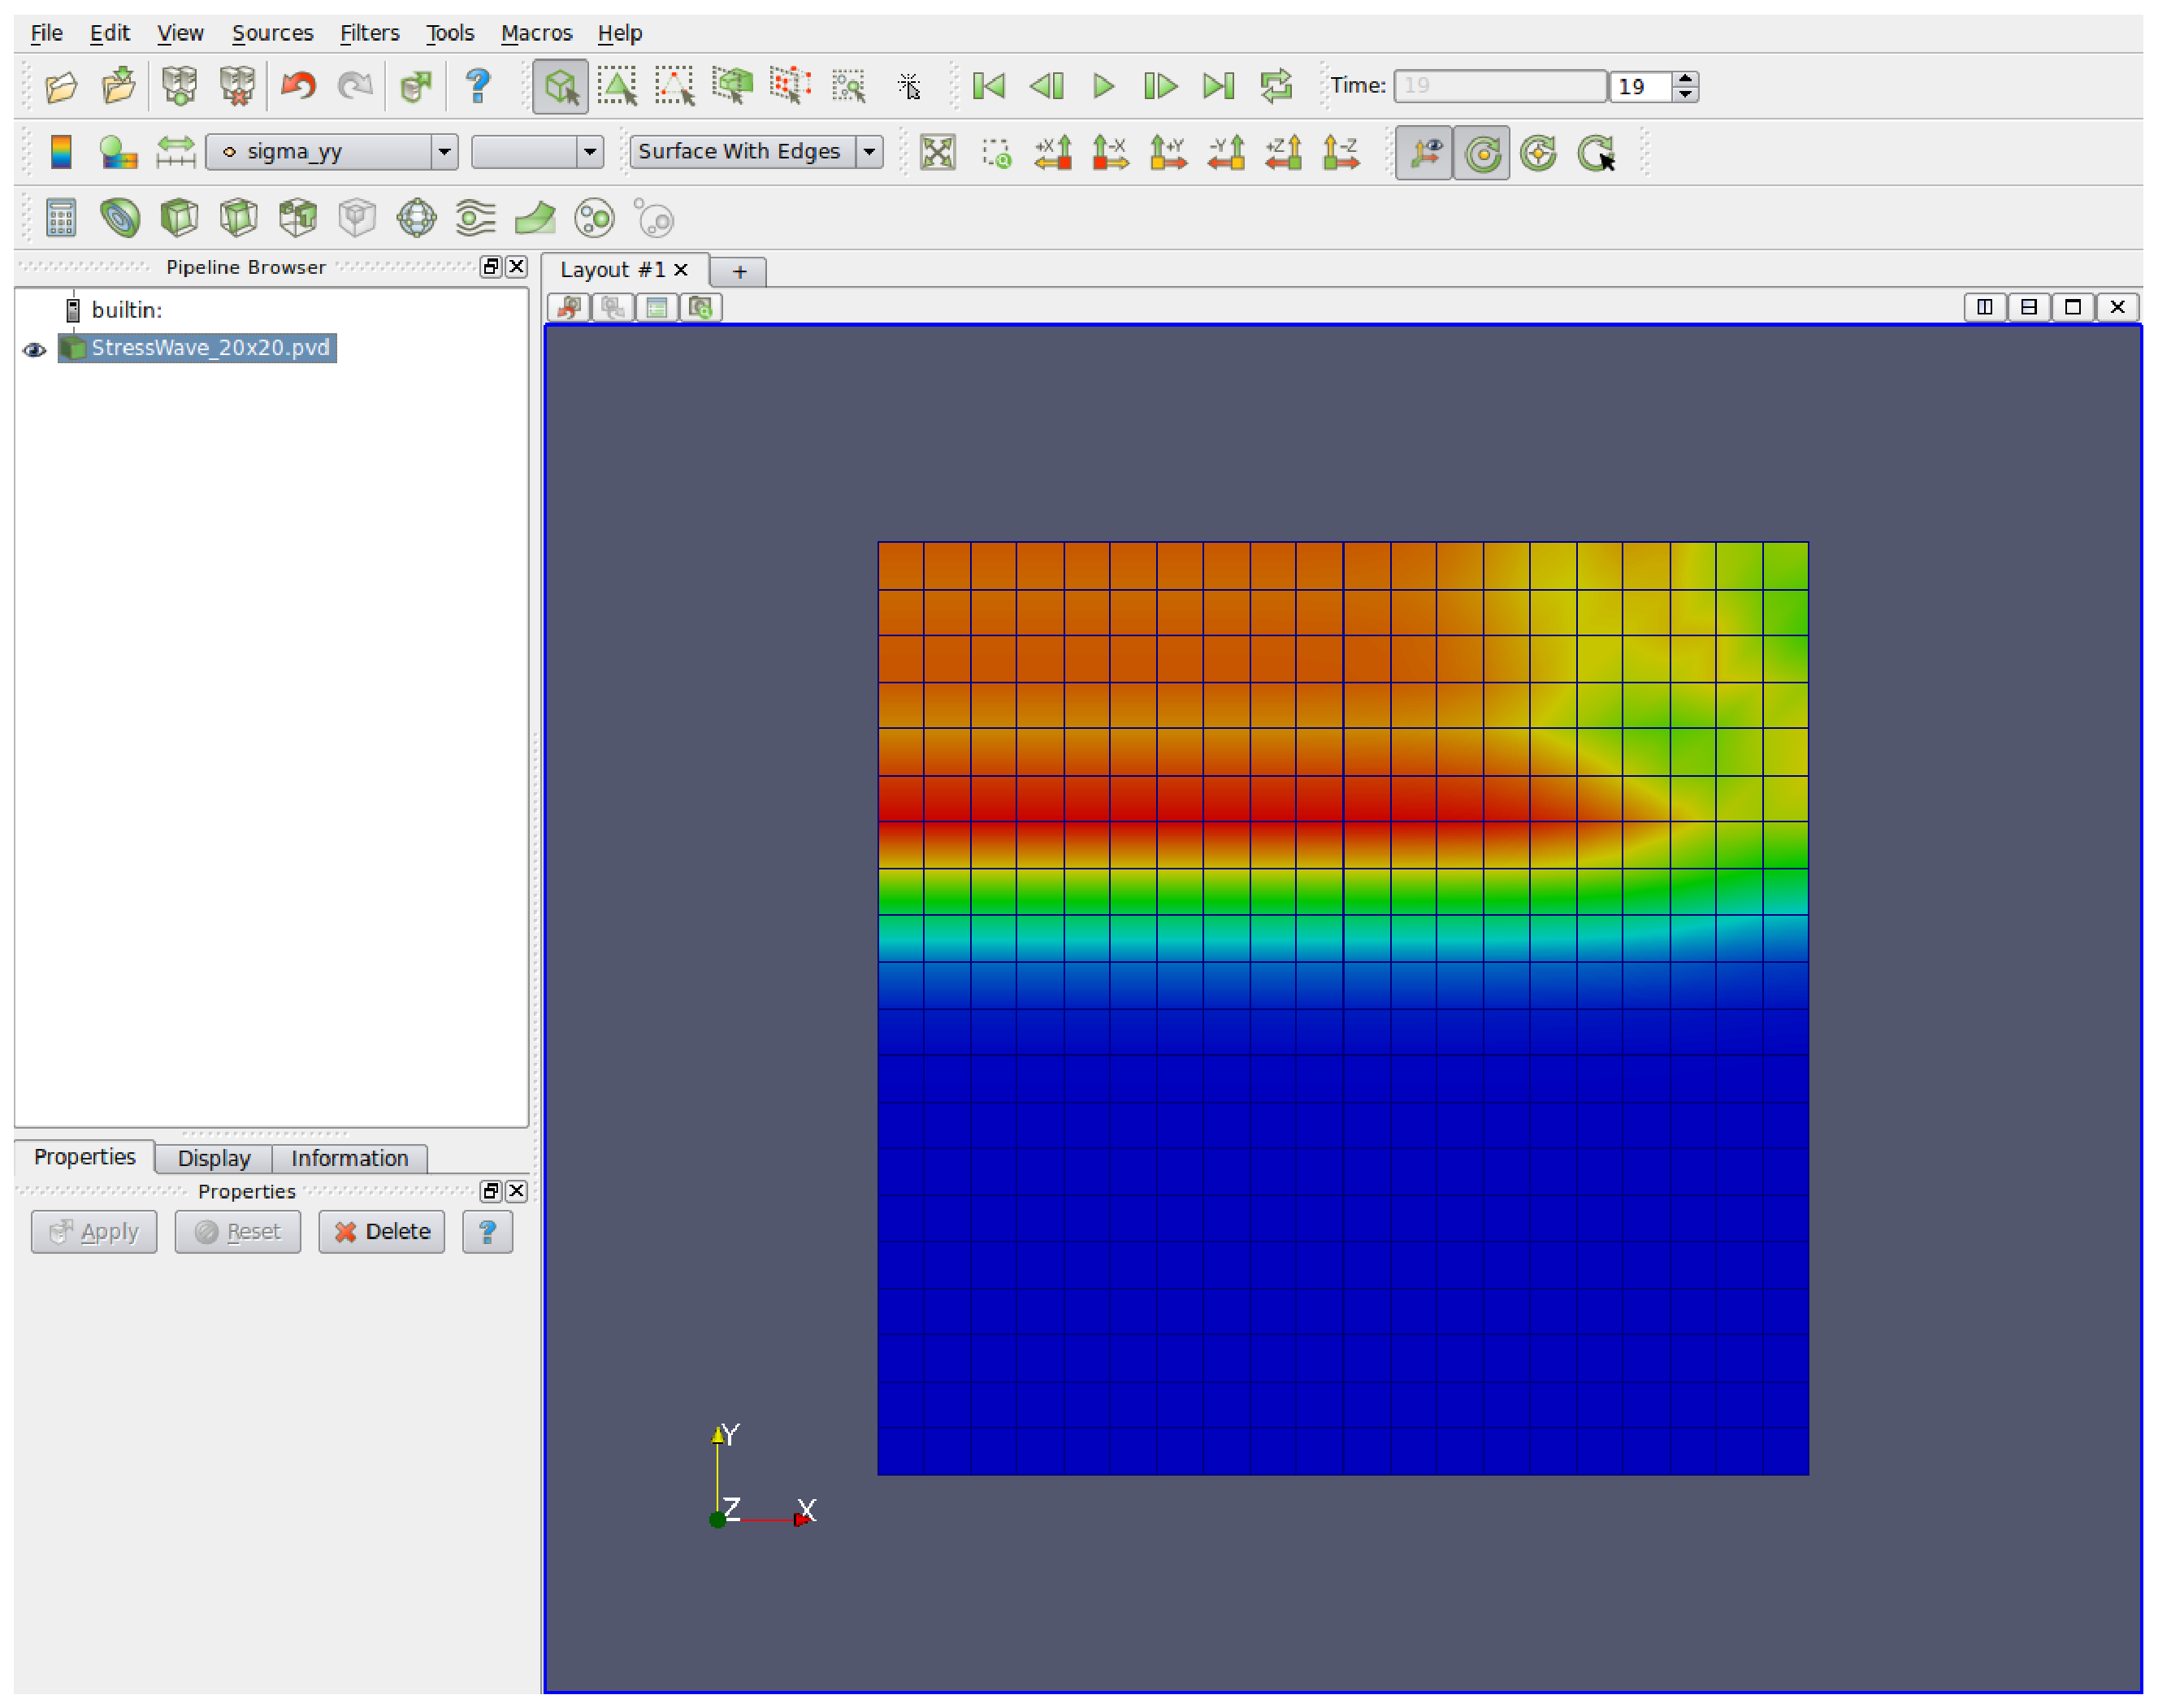
\includegraphics[width=0.6\textwidth]{img/screen.eps}
\caption{Screen shot of the results of the simulation \texttt{StressWave20x20.pro} shown in \textsc{Paraview}.}
\label{fig:stress}
\end{figure}

\section{Quick start}

In order to test whether everything is installed properly, the following two simulations can be run.

\subsection*{Simple example} 

In the directory \texttt{examples/ch02} the script \texttt{PatchTest.py} can be executed from a terminal (or DOS-shell) by typing:
\begin{verbatim}
  python PatchTest.py
\end{verbatim}
In Windows, this script can also be executed by double-clicking the icon.

\subsection*{\textsc{PyFEM} example} 

The full finite element code \progname~can be run by typing \texttt{pyfem} in the terminal. In directory \texttt{examples/ch04} for example,
the input file \texttt{ShallowTrussRiks.pro} is processed by typing:
\begin{verbatim}
  pyfem ShallowTrussRiks.pro
\end{verbatim}
Here, \texttt{ShallowTrussRiks.pro} is the input file, which by definition ends with \texttt{.pro}. When it is
opened in a text editor, it looks as follows:

\begin{graybox}
\begin{verbatim}
  input = "ShallowTrussRiks.dat";

  TrussElem  = 
  {
    ....
  };

  SpringElem =
  {
    ....
  };

  solver =
  {
    ....
  };

  outputModules = ["graph"];

  graph = 
  {
    ....
  };
\end{verbatim}
\end{graybox}
The dots indicate lines that have been omitted in this example.
The first argument in the \texttt{.pro}-file specifies the input file, which contains the positions of 
the nodes, the element connectivity and the boundary conditions. The structure of this file, which normally has 
the extension \texttt{.dat}, is as follows:
\begin{graybox}
\begin{verbatim}
  <Nodes>
    1   0.0 0.0 ;
    2 -10.0 0.0 ;
    3  10.0 0.0 ;
    4   0.0 0.5 ;
  </Nodes>

  <Elements>
    1 'TrussElem' 2 4 ;
    2 'TrussElem' 3 4 ;
    3 'SpringElem' 1 4 ;
  </Elements>

  <NodeConstraints>
    u[1] = 0.0;
    u[2] = 0.0;
    u[3] = 0.0;

    v[1] = 0.0;
    v[2] = 0.0;
    v[3] = 0.0;
  </NodeConstraints>

  <ExternalForces>
    v[4] = -100.0 ;
  </ExternalForces>
\end{verbatim}
\end{graybox}	
The nodes are defined between the labels \texttt{<Nodes>} and \texttt{</Nodes>}. The first number 
indicates the node identification number. The remaining numbers denote the coordinates in $x$-, $y$-, and in the 
case of a three dimensional simulation, the $z$-direction. For example, node 2 has the $x$ and $y$ coordinates $(-10,0)$.

The element connectivity is given after the tag \texttt{<Elements>}. 
The first number indicates the element ID number. The string refers to the name of the
element model this element belongs to. The remaining numbers are the nodes that are used to construct 
the element. In this example, the first element is of the type \texttt{'TrussElem'} and is supported
by nodes 2 and 4.

The boundary conditions and applied loads are specified next. The node constraints are given after the label \texttt{<NodeConstraints>}. 
In this example, the displacement components \texttt{u} and
\texttt{v} of nodes 1,2 and 3 have a prescribed value of 0.0. The external forces are specified in a 
similar manner in the field \texttt{<ExternalForces>}. Here, a unit external force with magnitude -100.0 is
added to node number 4 in the direction that corresponds to the \texttt{'v'} displacement. Hence, this force is
acting in the negative $y$-direction.

The parameters of the finite element model are specified in the \texttt{.pro} file, 
in the fields \texttt{TrussElem} and \texttt{SpringElem}, which refer to the labels used in the element connectivity
description.

\begin{graybox}
\begin{verbatim}
  TrussElem  = 
  {
    type = "Truss";
    E    = 5e6;
    Area = 1.0;
  };

  SpringElem =
  {
    type = "Spring";
    k    = 100.0;
  };
\end{verbatim}
\end{graybox}
The elements denoted by the label \texttt{TrussElem} are of the type \texttt{'Truss'}. This model requires two
additional parameters, the Young's modulus of the material \texttt{E} and the area of the cross-section \texttt{Area}.
The label \texttt{SpringElem} denote elements of the type \texttt{'Spring'}. Here, one additional parameter is required: the
spring stiffness \texttt{k}. A detailed overview of the element types and the corresponding parameters can be found in Section~\ref{sec:elements}
of this manual.

\vspace{2mm}
\noindent
The parameters of the solver are defined next:

\begin{graybox}
\begin{verbatim}
  solver =
  {
    type = 'RiksSolver';

    fixedStep = true;
    maxLam    = 10.0; 
  };
\end{verbatim}
\end{graybox}
The solver is of the type \texttt{'RikSolver'}. The two additional parameters specify that the magnitude of the path-parameter is
constant (\texttt{fixedStep = true}) and that the simulation is stopped when the load parameter $\lambda$ reaches a value of 10.0. 
A detailed overview of available solver types and their parameters is given in Section~\ref{sec:solver}.

Finally, the results of the simulation can be stored and visualised in several ways. To this end, a chain of output modules can be 
specified. In this example, the results are stored in a load-displacement curve in the module \texttt{GraphWriter}.

\begin{graybox}
\begin{verbatim}
  outputModules = ["graph"];

  graph =
  {
    type     = "GraphWriter";
    onScreen = true;

    columns = [ "disp" , "load" ];

    disp =
    {
      type   = "state";
      node   = 4;
      dof    = 'v';
      factor = -1.0;
    };
  
    load =
    { 
      type = "fint";
      node = 4;
      dof  = 'v';
    };
  };
\end{verbatim}
\end{graybox}
In this example, two colums are stored: \texttt{'disp'}, the displacement (\texttt{'state'}) of node 4 in the vertical 
direction and \texttt{'load'}, the corresponding internal force. The parameter \texttt{onScreen = true} is used
to show the load-displacement curve on the screen during the simulation. By default, the results will be stored in a file called
\texttt{ShallowTrussRiks.out}. A description of all available output 
modules can be found in Section~\ref{sec:output}.

\section{Solvers}\label{sec:solver}

In this section, a concise overview of the solvers that are available in \progname~is given.

\subsection{Linear solver}

The linear solver is discussed in detail in Section 2.6 of the book.

\begin{tabular}{p{20mm}p{74mm}}
Name:    & \texttt{LinearSolver} \\
Source:  & \texttt{pyfem/solver/LinearSolver.py} \\
\multicolumn{2}{l}{\textbf{Mandatory parameters:}} \\
~~None & \\
\multicolumn{2}{l}{\textbf{Optional parameters:}} \\ 
~~None & \\
\multicolumn{2}{l}{\textbf{Examples:}}\\
~~\texttt{ch02}: & \texttt{PatchTest4.pro}\\
~~\texttt{ch02}: & \texttt{PatchTest8.pro}
\end{tabular}

\subsection{Non-linear (Newton-Raphson) solver}

The Newton-Raphson solver can be used to solve non-linear systems
with a monotonously increasing external load or prescribed displacement. The
exact procedure is discussed in detail in Sections 2.4 and 2.5 of the book.

\vspace{2mm}
\begin{tabular}{p{22mm}p{74mm}}
Name:    & \texttt{NonlinearSolver} \\
Source:  & \texttt{pyfem/solver/NonlinearSolver.py} \\
\multicolumn{2}{l}{\textbf{Mandatory parameters:}} \\
~~None & \\
\multicolumn{2}{l}{\textbf{Optional parameters:}} \\ 
~~\texttt{maxLam}    & The maximum load parameter $\lambda$ for which the
                      ` simulation will be terminated.\\
~~\texttt{maxCycle}  & The number of load cycles (loading steps) after which the simulation will be terminated.\\
~~\texttt{tol}       & The precision that is used to determine whether a solution is converged. The 
                       default value is set to $10^{-3}$.\\
\multicolumn{2}{l}{\textbf{Examples:}}\\
~~\texttt{ch03}: & \texttt{cantilever8.pro}\\
~~\texttt{ch06}: & \texttt{ContDamExample.pro}
\end{tabular}

\subsection{Riks' arc-length solver}

Riks' arc-length method allows to solve problems in which the load parameter is not monotonously increasing. The
solver is discussed in detail in Section 4.2 of the book. The source code is explained in detail in Section 4.3.

\vspace{2mm}
\begin{tabular}{p{22mm}p{74mm}}
Name:    & \texttt{RiksSolver} \\
Source:  & \texttt{pyfem/solver/RiksSolver.py} \\
\multicolumn{2}{l}{\textbf{Mandatory parameters:}} \\
~~None & \\
\multicolumn{2}{l}{\textbf{Optional parameters:}} \\ 
~~\texttt{maxFactor} & The maximum for which the path-parameter
                       may increase with respect to the magnitude of the path-parameter
                       in the first step.\\
~~\texttt{fixedStep} & If set to \texttt{true} a constant step size is used. This is identical to
                       \texttt{maxFactor=1}. The default value is \texttt{false}.\\
~~\texttt{opt}       & Optimal number of iterations, see Section 4.5 of the book for further details.\\
~~\texttt{tol}       & The precision that is used to determine whether a solution is converged. The 
                       default value is set to $10^{-3}$.\\
~~\texttt{maxLam}    & The maximum load parameter $\lambda$ for which the
                      ` simulation will be terminated.\\
\multicolumn{2}{l}{\textbf{Examples:}}\\
~~\texttt{ch04}: & \texttt{ShallowTrussRiks.pro}\\
~~\texttt{ch09}: & \texttt{FrameKirchhoff.pro}\\
~~\texttt{ch09}: & \texttt{FrameTimoshenko.pro}\\
~~\texttt{ch09}: & \texttt{KirchhoffEuler\_01.pro}\\
~~\texttt{ch09}: & \texttt{KirchhoffEuler\_1.pro}\\
~~\texttt{ch09}: & \texttt{KirchhoffEuler.pro}
\end{tabular}

\subsection{Dissipated energy solver}

This is the dissipated energy based arc-length solver as described in Section 4.2, page 123 of the book.

\vspace{2mm}
\begin{tabular}{p{22mm}p{74mm}}
Name:         & \texttt{DissipatedEnergySolver} \\
Source:  & \texttt{pyfem/solver/DissipatedEnergySolver.py} \\
\multicolumn{2}{l}{\textbf{Mandatory parameters:}} \\
~~\texttt{switchEnergy} & Amount of dissipated energy in a single step for which the solution technique will switch from
                          force controlled to energy dissipation controlled.\\
\multicolumn{2}{l}{\textbf{Optional parameters:}} \\ 
~~\texttt{maxCycle} &  Number of cycles after which the simulation will be terminated.\\
~~\texttt{maxdTau}  &  Maximum amount of energy that may be dissipated in a single step.\\
~~\texttt{tol}      &  The precision that is used to determine whether a solution is converged. The 
                       default value is set to $10^{-3}$.\\
~~\texttt{maxLam}    & The maximum load parameter $\lambda$ for which the
                      ` simulation will be terminated.\\
\multicolumn{2}{l}{\textbf{Examples:}}\\
~~\texttt{ch13}: & \texttt{PeelTest.pro}
\end{tabular}

\subsection{Explicit time integration solver}

The explicit time integration solver is discussed in detail in Section 5.2 of the book. The source code is explained in detail in Section 5.3 of the book.

\vspace{2mm}
\begin{tabular}{p{22mm}p{74mm}}
Name:         & \texttt{ExplicitSolver} \\
Source:  & \texttt{pyfem/solver/ExplicitSolver.py} \\
\multicolumn{2}{l}{\textbf{Mandatory parameters:}} \\
~~\texttt{dtime} & Magnitude of time step\\
~~\texttt{lam}   & Load factor $\lambda$ as a function of time. This can be written
                 as a string. For example, \texttt{'4.0*sin(3.0*t)'} represents a sinusoidal 
                 load, with period 3.0 and amplitude 4.0.	\\
\multicolumn{2}{l}{\textbf{Optional parameters:}} \\ 
~~\texttt{maxCycle} &  Number of cycles after which the simulation will be terminated.\\
~~\texttt{maxTime}  &  Time after which the simulation will be terminated.\\
\multicolumn{2}{l}{\textbf{Examples:}}\\
~~\texttt{ch05}: & \texttt{StressWave20x20.pro}
\end{tabular}

\section{Output modules}\label{sec:output}

\subsection{Contour writer}

The output of a selected number of nodes is stored in a multi column file by this writer. For each step in the simulation a
new file will be written ithe following format:

\noindent
\texttt{filename-contour-stepnumber.out}

The columns contain the nodeIDs, the $x$ and $y$ coordinates of the node, the displacements, stresses and the tractions.

\vspace{2mm}
\begin{tabular}{p{22mm}p{74mm}}
Name:         & \texttt{ContourWriter} \\
Source:  & \texttt{pyfem/io/ContourWriter.py} \\
\multicolumn{2}{l}{\textbf{Mandatory parameters:}} \\
~~\texttt{nodes}    & An array of nodes.\\
\multicolumn{2}{l}{\textbf{Examples:}}\\
~~\texttt{ch13}: & \texttt{PeelTest40.pro}
\end{tabular}

\subsection{Mesh output writer}\label{par:vtk}

The mesh output writer saves all data during a simulation to the disk.
The data is organised as follows: during a simulation, a single output file \texttt{filename.pvd} will be created which refers to the output
of single steps, which are stored in the file \texttt{filename-xx.vtu}, where \texttt{xx} indicates the step number.
This data can be visualised by opening the file \texttt{filename.pvd} in the external program \textsc{Paraview}.

\vspace{2mm}
\begin{tabular}{p{22mm}p{74mm}}
Name:         & \texttt{MeshWriter} \\
Source:  & \texttt{pyfem/io/MeshWriter.py} \\
\multicolumn{2}{l}{\textbf{Mandatory parameters:}} \\
~~None  & \\
\multicolumn{2}{l}{\textbf{Optional parameters:}} \\ 
~~\texttt{prefix} & The prefix of the output filename that will be used. By default, the prefix of the 
                    input filename is used.\\
~~\texttt{interval} & The interval (number of cycles) for which output is stored. By default, every step is
                    stored.\\
~~\texttt{elementgroup} & When specified, only the elements in this group will be stored. By default, all elements
                    will be stored.\\
\multicolumn{2}{l}{\textbf{Examples:}}\\
~~\texttt{ch03}: & \texttt{cantilever8.pro}\\
~~\texttt{ch05}: & \texttt{StressWave20x20.pro}\\
~~\texttt{ch06}: & \texttt{ContDamExample.pro}\\
~~\texttt{ch13}: & \texttt{PeelTest.pro}
\end{tabular}

\subsection{Graph output writer}

The output is stored in a multi column file by this writer. The first two columns can be shown on the screen as a curve during
the simuluation.

\vspace{2mm}
\begin{tabular}{p{22mm}p{74mm}}
Name:         & \texttt{GraphWriter} \\
Source:  & \texttt{pyfem/io/GraphWriter.py} \\
\multicolumn{2}{l}{\textbf{Mandatory parameters:}} \\
~~\texttt{columns} & Array of strings indicating the column that will be stored. For each column,
                   the type of data, and if needed, the node, degree of freedom and scaling factor needs to be specified.\\
~~\texttt{type}    & Type of data. This can be either \texttt{state}, \texttt{velo}, \texttt{fint}, \texttt{stress}, etc.\\
~~\texttt{node}    & Node ID.\\
~~\texttt{dof}     & Degree of freedom. This is most likely \texttt{'u'} or \texttt{'v'}\\
\multicolumn{2}{l}{\textbf{Optional parameters:}} \\ 
~~\texttt{factor} & The scaling factor for the output. The default value is 1.0.\\
~~\texttt{onScreen} & When set to \texttt{true} the first two columns will be shown on the screen. The default value is \texttt{false}.\\
\multicolumn{2}{l}{\textbf{Examples:}}\\
~~\texttt{ch04}: & \texttt{ShallowTrussRiks.pro}\\
~~\texttt{ch06}: & \texttt{ContDamExample.pro}\\
~~\texttt{ch09}: & \texttt{FrameKirchhoff.pro}\\
~~\texttt{ch09}: & \texttt{FrameTimoshenko.pro}\\
~~\texttt{ch09}: & \texttt{KirchhoffEuler\_01.pro}\\
~~\texttt{ch09}: & \texttt{KirchhoffEuler\_1.pro}\\
~~\texttt{ch09}: & \texttt{KirchhoffEuler.pro}\\
~~\texttt{ch13}: & \texttt{PeelTest.pro}
\end{tabular}

%\subsection{General output writer}

%In this writer, all data is saved on a disk.
%\begin{tabular}{p{22mm}p{74mm}}
%Name:         & \texttt{OutputWriter} \\
%Source:  & \texttt{pyfem/io/outputWriter.py} \\
%\multicolumn{2}{l}{\textbf{Mandatory parameters:}} \\
%~~\texttt{columns} & Array of strings indicating the column that will be stored. For each column,
%                   the type of data, and if needed, the node, degree of freedom and scaling factor\\
%~~\texttt{type}    & Type of data. This can be either \texttt{state},\texttt{velo},\texttt{fint},\texttt{stress},etc.\\
%~~\texttt{node}    & Node ID.\\
%~~\texttt{dof}     & Degree of freedom. This is most likely \texttt{'u'} or \texttt{'v'}\\
%\multicolumn{2}{l}{\textbf{Optional parameters:}} \\ 
%~~\texttt{factor} & The scaling factor for the output. The default value is 1.0.\\
%\multicolumn{2}{l}{\textbf{Examples:}}\\
%~~\texttt{ch05}: & \texttt{StressWave20x20.pro}
%\end{tabular}

\section{Elements}\label{sec:elements}

In this section, a list of elements available in \progname~is given.

\subsection{Finite strain continuum}

The finite strain continuum element is discussed in detail in Section 3.6 of the book. In the code, the two dimensional
version is implemented. It can be used as a 3,4,6,8 and 9 node element.

\vspace{2mm}
\begin{tabular}{p{22mm}p{74mm}}
Name:         & \texttt{FiniteStrainContinuum} \\
Source:  & \texttt{pyfem/materials/FiniteStrainContinuum.py} \\
\multicolumn{2}{l}{\textbf{Mandatory parameters:}} \\
~~\texttt{material} & The material model that is used in this element, see Section~\ref{sec:matmodel} for more details.\\
\multicolumn{2}{l}{\textbf{Optional parameters:}} \\ 
~~None  & \\
\multicolumn{2}{l}{\textbf{Examples:}}\\
~~\texttt{ch03}: & \texttt{cantilever8.pro}\\
~~\texttt{ch05}: & \texttt{StressWave20x20.pro}
\end{tabular}

\subsection{Kirchhoff non-linear beam}

The Kirchhoff beam element is discussed in Section 9.2.

\vspace{2mm}
\begin{tabular}{p{22mm}p{74mm}}
Name:         & \texttt{KirchhoffBeam} \\
Source:  & \texttt{pyfem/elements/KirchhoffBeam.py} \\
\multicolumn{2}{l}{\textbf{Mandatory parameters:}} \\
~~\texttt{E} & Young's modulus\\
~~\texttt{A} & Cross-section of the truss\\
~~\texttt{I} & Moment of inertia\\
\multicolumn{2}{l}{\textbf{Optional parameters:}} \\ 
~~None  & \\
\multicolumn{2}{l}{\textbf{Examples:}}\\
~~\texttt{ch09}: & \texttt{FrameKirchhoff.pro}
\end{tabular}

\subsection{Plate element}

A simple implementation of a first order shear plate element is implement. This 
element is not discussed in the book.

\vspace{2mm}
\begin{tabular}{p{22mm}p{74mm}}
Name:         & \texttt{Plate} \\
Source:  & \texttt{pyfem/elements/Plate.py} \\
\multicolumn{2}{l}{\textbf{Mandatory parameters:}} \\
~~\texttt{materials} & A list of the material that are used in the stacking sequence.\\
~~\texttt{layers} & A list of possible layers (materials, orientation and thicknesses).\\
~~\texttt{stack} & An array with the order in which the layers are stacked.\\
\multicolumn{2}{l}{\textbf{Optional parameters:}} \\ 
~~None  & \\
\multicolumn{2}{l}{\textbf{Examples:}}\\
~~\texttt{plate}: & \texttt{plate_test_06.pro}
\end{tabular}

\subsection{Small strain continuum}

The small strain continuum element is discussed in detail in Section 2.6 of the book. In the code, the two dimensional
version is implemented. It can be used as a 3,4,6,8 and 9 node element.

\vspace{2mm}
\begin{tabular}{p{22mm}p{74mm}}
Name:         & \texttt{SmallStrainContinuum} \\
Source:  & \texttt{pyfem/materials/SmallStrainContinuum.py} \\
\multicolumn{2}{l}{\textbf{Mandatory parameters:}} \\
~~\texttt{material} & Material Model, see Section~\ref{sec:matmodel} \\
\multicolumn{2}{l}{\textbf{Optional parameters:}} \\ 
~~None  & \\
\multicolumn{2}{l}{\textbf{Examples:}}\\
~~\texttt{ch02}: & \texttt{PatchTest4.pro}\\
~~\texttt{ch02}: & \texttt{PatchTest8.pro}\\
~~\texttt{ch06}: & \texttt{ContDamExample.pro}\\
~~\texttt{ch13}: & \texttt{PeelTest.pro}
\end{tabular}

\subsection{Linear spring}

The linear spring is used in the Shallow Truss examples in the first chapters of the book.

\vspace{2mm}
\begin{tabular}{p{22mm}p{74mm}}
Name:         & \texttt{Spring} \\
Source:  & \texttt{pyfem/elements/Spring.py} \\
\multicolumn{2}{l}{\textbf{Mandatory parameters:}} \\
~~\texttt{k} & Spring stiffness\\
\multicolumn{2}{l}{\textbf{Optional parameters:}} \\ 
~~None  & \\
\multicolumn{2}{l}{\textbf{Examples:}}\\
~~\texttt{ch04}: & \texttt{ShallowTrussRiks.pro}
\end{tabular}

\subsection{Timoshenko non-linear beam}

The Timoshenko beam element is discussed in Section 9.2 of the book.

\vspace{2mm}
\begin{tabular}{p{22mm}p{74mm}}
Name:         & \texttt{TimoshenkoBeam} \\
Source:  & \texttt{pyfem/elements/TimoshenkoBeam.py} \\
\multicolumn{2}{l}{\textbf{Mandatory parameters:}} \\
~~\texttt{E} & Young's modulus\\
~~\texttt{A} & Cross-section of the truss\\
~~\texttt{I} & Moment of intertia\\
~~\texttt{G} & Shear modulus\\
\multicolumn{2}{l}{\textbf{Optional parameters:}} \\ 
~~None  & \\
\multicolumn{2}{l}{\textbf{Examples:}}\\
~~\texttt{ch09}: & \texttt{FrameTimoshenko.pro}
\end{tabular}


\subsection{Non-linear truss}

The non-linear truss element is discussed in Sections 3.1 and 3.2 of the book.

\vspace{2mm}
\begin{tabular}{p{22mm}p{74mm}}
Name:         & \texttt{Truss} \\
Source:  & \texttt{pyfem/elements/Truss.py} \\
\multicolumn{2}{l}{\textbf{Mandatory parameters:}} \\
~~\texttt{E} & Young's modulus\\
~~\texttt{A} & Cross-section of the truss\\
\multicolumn{2}{l}{\textbf{Optional parameters:}} \\ 
~~None  & \\
\multicolumn{2}{l}{\textbf{Examples:}}\\
~~\texttt{ch04}: & \texttt{ShallowTrussRiks.pro}
\end{tabular}

\subsection{Cohesive zone interface}

The Cohesive zone interface element is discussed in Section 13.2 of the book.

\vspace{2mm}
\begin{tabular}{p{22mm}p{74mm}}
Name:         & \texttt{Interface} \\
Source:  & \texttt{pyfem/materials/Interface.py} \\
\multicolumn{2}{l}{\textbf{Mandatory parameters:}} \\
~~\texttt{material} & Material Model, see Section~\ref{sec:matmodel} \\
\multicolumn{2}{l}{\textbf{Optional parameters:}} \\ 
~~\texttt{intmethod}  & Integration method, this can be either \texttt{Gauss}, \texttt{Newton-Cotes} or \texttt{Lobatto}. The default is \texttt{Newton-Cotes}\\
~~\texttt{intorder}   & Integration order. The level of over- or underintegration is specified here as an integer (e.g. \texttt{+2} or \texttt{-1}). Default value is \texttt{0}.\\
\multicolumn{2}{l}{\textbf{Examples:}}\\
~~\texttt{ch13}: & \texttt{TractionOscillation.pro}\\
~~\texttt{ch13}: & \texttt{PeelTest.pro}
\end{tabular}

\subsection{Solid-like shell}

This solid-like shell element is based on Hashagen's implementation. The current
implementation only allows for a 8 node element and can be used in combination 
with a Linear solver.

\vspace{2mm}
\begin{tabular}{p{22mm}p{74mm}}
Name:         & \texttt{SLS} \\
Source:  & \texttt{pyfem/elemtents/SLS.py} \\
\multicolumn{2}{l}{\textbf{Mandatory parameters:}} \\
~~\texttt{material} & Material Model, see Section~\ref{sec:matmodel} \\
\multicolumn{2}{l}{\textbf{Optional parameters:}} \\ 
~~\texttt{layers}  & The layer stacking. For each layer, the orientation \texttt{angle}, the
 relative thickness (\texttt{thickness}) and the material type \texttt{material} needs to be specified.\\
~~\texttt{sls}: & Several examples
\end{tabular}
\section{Material models}\label{sec:matmodel}

In this section, the input parameters for the different material models that are available in
\progname~are given.

\subsection{Plane strain linear elastic model}

A plane strain, linear elastic constitutive relation as presented on page 109-110 of the book.\\

\begin{tabular}{p{22mm}p{74mm}}
Name:         & \texttt{PlaneStrain} \\
Source:  & \texttt{pyfem/materials/PlaneStrain.py} \\
\multicolumn{2}{l}{\textbf{Mandatory parameters:}} \\
~~\texttt{E} & Young's modulus \\
~~\texttt{nu} & Poisson's ratio \\
\multicolumn{2}{l}{\textbf{Optional parameters:}} \\ 
~~None  & \\
\multicolumn{2}{l}{\textbf{Examples:}}\\
~~\texttt{ch02}: & \texttt{PatchTest4.pro}\\
~~\texttt{ch02}: & \texttt{PatchTest8.pro}\\
~~\texttt{ch05}: & \texttt{StressWave20x20.pro}\\
~~\texttt{ch13}: & \texttt{TractionOscillation.pro}\\
~~\texttt{ch13}: & \texttt{PeelTest.pro}
\end{tabular}

\subsection{Plane strain damage}

See Section 6.2 in the book for a detailed description.\\

\begin{tabular}{p{22mm}p{74mm}}
Name:         & \texttt{PlaneStrainDamage} \\
Source:  & \texttt{pyfem/materials/PlaneStrainDamage.py} \\
\multicolumn{2}{l}{\textbf{Mandatory parameters:}} \\
~~\texttt{E} & Young's modulus \\
~~\texttt{nu} & Poisson's ratio \\
~~\texttt{kappa0} & Equivalent strain at which damage intiates.\\
~~\texttt{kappac} & Equivalent strain at which damage is 1.0.\\
\multicolumn{2}{l}{\textbf{Optional parameters:}} \\
~~None  & \\
\multicolumn{2}{l}{\textbf{Examples:}}\\
~~\texttt{ch06}: & \texttt{ContDamExample.pro}
\end{tabular}

\subsection{Plane stress linear elastic}

\begin{tabular}{p{22mm}p{74mm}}
Name:         & \texttt{PlaneStrain} \\
Source:  & \texttt{pyfem/materials/PlaneStrain.py} \\
\multicolumn{2}{l}{\textbf{Mandatory parameters:}} \\
~~\texttt{E} & Young's modulus \\
~~\texttt{nu} & Poisson's ratio \\
\multicolumn{2}{l}{\textbf{Optional parameters:}} \\ 
~~None  & \\
\multicolumn{2}{l}{\textbf{Examples:}}
\end{tabular}

\subsection{Isotropic}

\begin{tabular}{p{22mm}p{74mm}}
Name:         & \texttt{Isotropic} \\
Source:  & \texttt{pyfem/materials/Isotropic.py} \\
\multicolumn{2}{l}{\textbf{Mandatory parameters:}} \\
~~\texttt{E} & Young's modulus \\
~~\texttt{nu} & Poisson's ratio \\
\multicolumn{2}{l}{\textbf{Optional parameters:}} \\ 
~~None  & \\
\multicolumn{2}{l}{\textbf{Examples:}}
\end{tabular}

\subsection{Transverse Isotropic}

\begin{tabular}{p{22mm}p{74mm}}
Name:         & \texttt{TransverseIsotropic} \\
Source:  & \texttt{pyfem/materials/TransverseIsotropic.py} \\
\multicolumn{2}{l}{\textbf{Mandatory parameters:}} \\
~~\texttt{E1}   & Young's modulus in longitudinal direction \\
~~\texttt{E2}   & Young's modulus in transverse direction \\
~~\texttt{nu12} & Poisson's ratio \\
~~\texttt{G12}  & Shear modulus \\
\multicolumn{2}{l}{\textbf{Optional parameters:}} \\ 
~~None  & \\
\multicolumn{2}{l}{\textbf{Examples:}}
\end{tabular}

\subsection{Sandwich Core}

\begin{tabular}{p{22mm}p{74mm}}
Name:         & \texttt{SandwichCore} \\
Source:  & \texttt{pyfem/materials/SandwichCore.py} \\
\multicolumn{2}{l}{\textbf{Mandatory parameters:}} \\
~~\texttt{E3}   & Young's modulus in thickness direction \\
~~\texttt{G13}  & Shear modulus in transverse 1-3 direction \\
~~\texttt{G23}  & Shear modulus in transverse 2-3 direction \\
\multicolumn{2}{l}{\textbf{Optional parameters:}} \\ 
~~\texttt{factor} & Multiplication factor for in-plane terms (default = 0.001)\\
\multicolumn{2}{l}{\textbf{Examples:}}
\end{tabular}

\subsection{Power Law cohesive model}

\begin{tabular}{p{22mm}p{74mm}}
Name:         & \texttt{PowerLawModeI} \\
Source:  & \texttt{pyfem/materials/PowerLawModeI.py} \\
\multicolumn{2}{l}{\textbf{Mandatory parameters:}} \\
~~\texttt{Tult} & Ultimate traction\\
~~\texttt{Gc} & Fracture toughness \\
\multicolumn{2}{l}{\textbf{Optional parameters:}} \\ 
~~None  & \\
\multicolumn{2}{l}{\textbf{Examples:}}\\
~~\texttt{ch13}: & \texttt{PeelTest.pro}
\end{tabular}

\subsection{Thouless Mode-I cohesive model}

\begin{tabular}{p{22mm}p{74mm}}
Name:         & \texttt{ThoulessModeI} \\
Source:  & \texttt{pyfem/materials/ThoulessModeI.py} \\
\multicolumn{2}{l}{\textbf{Mandatory parameters:}} \\
~~\texttt{Tult} & Ultimate traction\\
~~\texttt{Gc}   & Fracture toughness \\
~~\texttt{d1d2} & The ratio between critical distances $d_1$ and $d_2$\\
~~\texttt{d1d3} & The ratio between critical distances $d_1$ and $d_3$\\
\multicolumn{2}{l}{\textbf{Optional parameters:}} \\ 
~~None  & \\
\multicolumn{2}{l}{\textbf{Examples:}}\\
~~\texttt{ch13}: & \texttt{PeelTestThouless.pro}
\end{tabular}

\subsection{Xu-Needleman cohesive model}

\begin{tabular}{p{22mm}p{74mm}}
Name:         & \texttt{XuNeedleman} \\
Source:  & \texttt{pyfem/materials/XuNeedleman.py} \\
\multicolumn{2}{l}{\textbf{Mandatory parameters:}} \\
~~\texttt{Tult} & Ultimate traction\\
~~\texttt{Gc} & Fracture toughness \\
\multicolumn{2}{l}{\textbf{Optional parameters:}} \\ 
~~None  & \\
\multicolumn{2}{l}{\textbf{Examples:}}\\
~~\texttt{ch13}: & \texttt{PeelTestXN.pro}
\end{tabular}

\section{Version history}

\begin{tabular}{p{5mm}p{27mm}p{75mm}}
0.1 & June 22, 2012 &
$\bullet$ Initial release \\
0.2 & June 28, 2012 &
$\bullet$ Introduction of \texttt{"All"} element group \\
    & &
$\bullet$ Robust parser for elements and nodes.\\
   & &
$\bullet$ Non-continuous node numbering in MeshWriter.\\
 & &
$\bullet$ Fixed material manager.\\
 & &
$\bullet$ Extended manual.\\
0.3 & July 5, 2012 & 
$\bullet$ Improved Windows set-up script.\\
0.4 & July 26, 2012 & 
$\bullet$ Extended GraphWriter.\\
0.7 & August 13, 2012 & 
$\bullet$ Added examples in Chapter 3 and 6. \\
 & & 
$\bullet$ General clean-up of the code.\\
0.8 & August 14, 2012 & 
$\bullet$ Extended user manual.\\
0.8.1 & August 17, 2012 &
$\bullet$ Updated Mac OS install script.\\
0.9 &  August 27, 2012 &
$\bullet$ Added 3, 6 and 9 node shape functions.\\
 & & 
$\bullet$ Added interface element.\\
  & &
$\bullet$ Added Dissipated Energy solver.\\
1.0 &  August 29, 2012 &
$\bullet$ First major release.\\
3.0 &  January 13, 2018 &
$\bullet$ Migration to Python 3.\\
3.0.1 &  October 14, 2018 &
$\bullet$ Bugfix to restore writing to console under Windows.\\
3.0.2 &  October 21, 2018 &
$\bullet$ Bugfix to find correct Scipy library.\\

\end{tabular}

\end{document}
